\section{Apéndices}
%En el ap´endice A se incluir´a el enunciado del TP. En el ap´endice B se incluir´an los
%c´odigos fuente de las funciones relevantes desde el punto de vista num´erico. Resultados
%que valga la pena mencionar en el trabajo pero que sean demasiado espec´ıficos para
%aparecer en el cuerpo principal del trabajo podr´an mencionarse en sucesivos ap´endices
%rotulados con las letras mayusculas del alfabeto romano. Por ejemplo: la demostraci´on
%de una propiedad que aplican para optimizar el algoritmo que programaron para resolver
%un problema.

\subsection{Apéndice A: Enunciado}
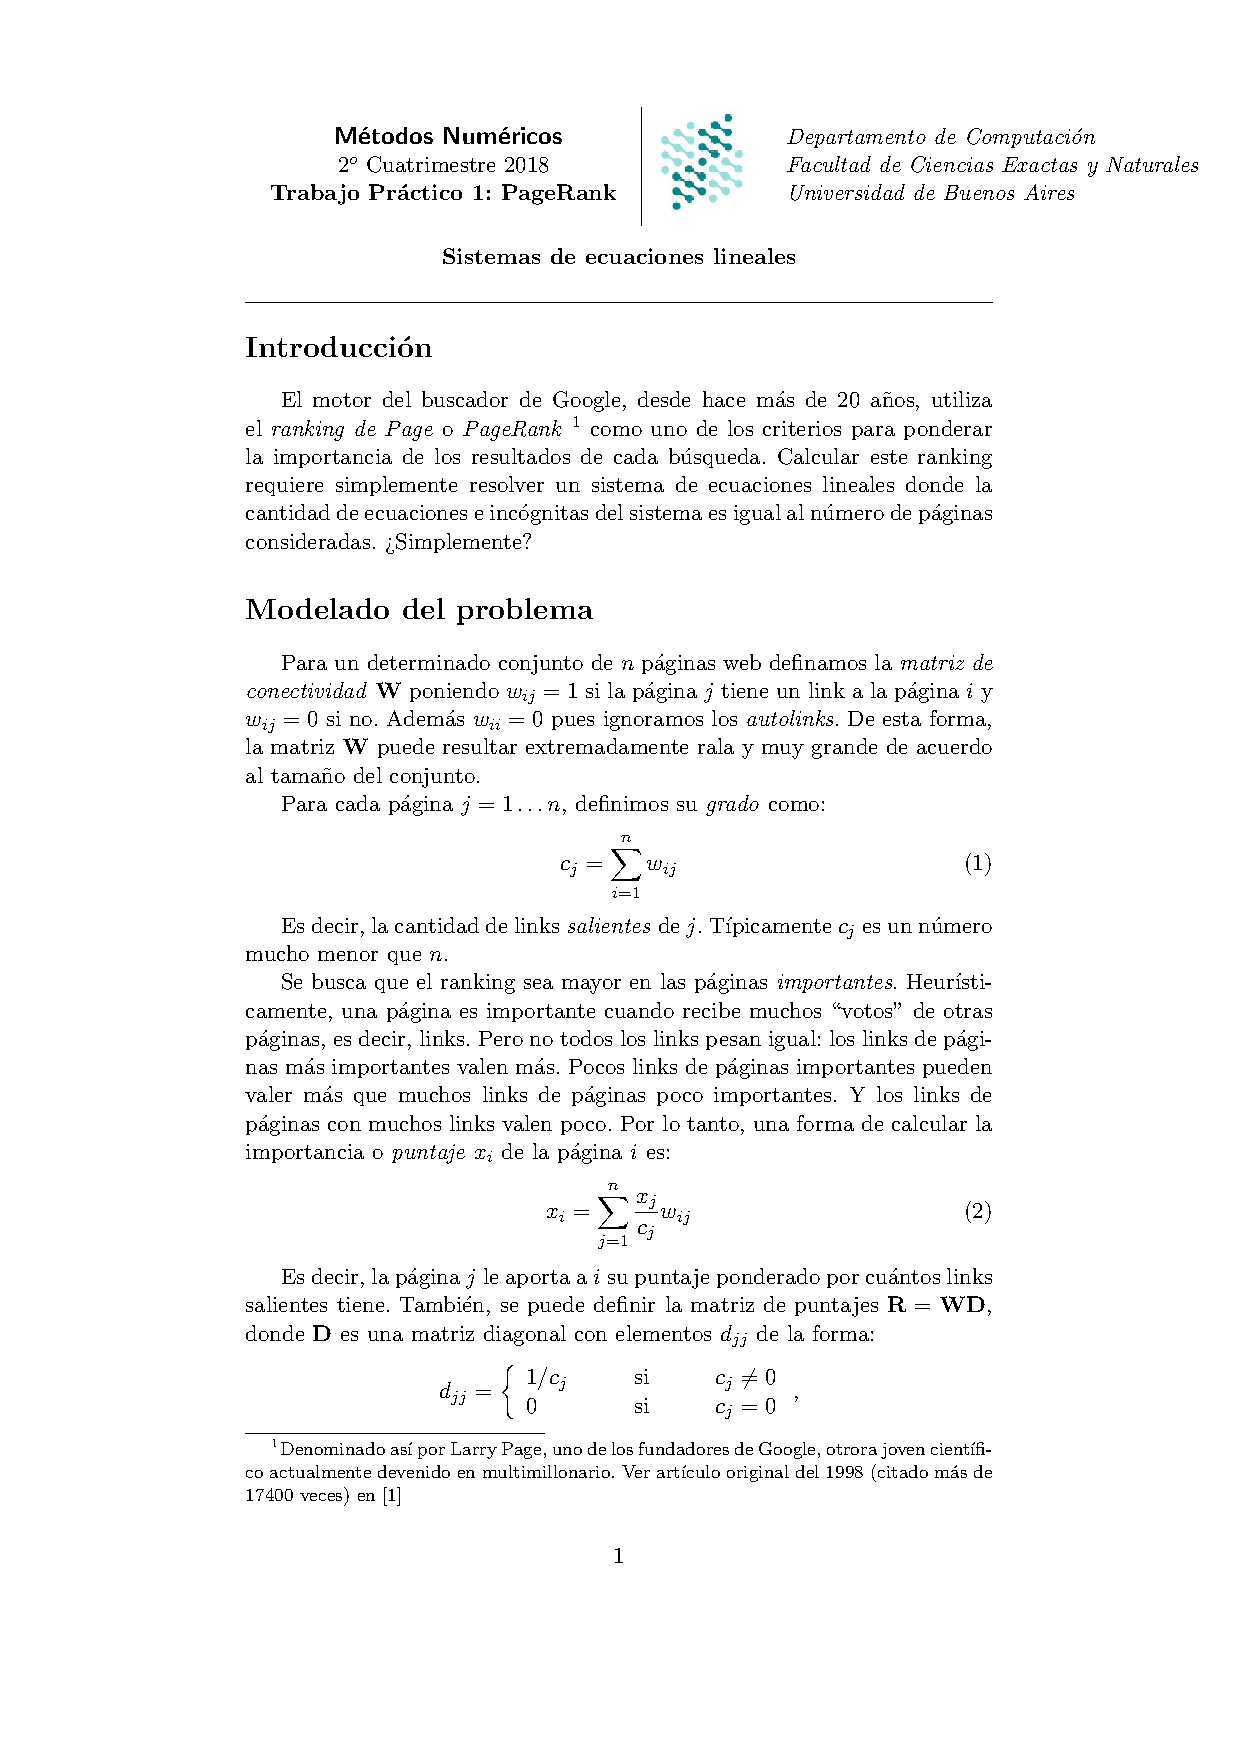
\includepdf[pages=-]{../tp1.pdf}

\subsection{Apéndice B: Código fuente relevante numéricamente}
Agregamos el código usado para resolver el sistema (método resolver de MatrizRala).
\begin{lstlisting}
vector<ld> MatrizRala::resolver(ll gamma) {
    vector<ld> b(this->filas.size(), gamma);

    // Eliminacion gaussiana
    for (unsigned int i = 0; i < this->filas.size() - 1; i++) {
        for (unsigned int j = i + 1; j < this->filas.size(); j++) {
            this->restarFila(i, j, b);
        }
    }

    // Sustituyo para atras
    vector<ld> x;
    x.push_back(b.back() / this->elem(this->filas.size() - 1, this->filas.size() - 1));
    for (int i = this->filas.size() - 2; i >= 0; i--) {
        ld sum = 0;

        for (unsigned int j = i + 1; j < this->filas.size(); j++) {
            sum += this->elem(i, j) * x[this->filas.size() - j - 1];
        }
        x.push_back((b[i] - sum) / this->elem(i, i));
    }

    reverse(x.begin(), x.end());
    this->normalizar(x);
    return x;
}
\end{lstlisting}

\subsection{Apéndice C: Demostración A e.d.d. $\Rightarrow A$ inversible}

Si $A=((a_{i,j})_{i,j\in [1,n]})$ es una matriz de diagonal estrictamente dominante, entonces A es inversible \\
\underline{Demostraci\'on:} \\
Por contrarrecíproco:  Supongamos que $A$ no es inversible, entonces su núcleo no se reduce a cero, existe entonces un vector: $X =	\begin{pmatrix}
							x_{1} \\
                            x_{2} \\
							\vdots \\
							x_{n} \\
						\end  {pmatrix}\not= 0 $ tal que  $AX = 0$. \newline
						\\
Entonces, se tiene que:
\begin{equation*}
\forall j \in [1,n], \displaystyle\sum_{\substack{i = 1}}^n a_{i,j} x_{j}= 0
\end{equation*}
 \newline
Como $X \not= 0$, existe $x_{k} \not= 0$ tal que
$| x_{k} |  = \max\{{ |x_{i}|, i \in [1,n] }\}$.\newline
Tenemos:  $-a_{k,k} x_{k} =  \displaystyle\sum_{\substack{i = 1\\i\neq k}}^n a_{i,k} x_{i}$ , de donde $|a_{k,k} x_{k}| \leq \displaystyle\sum_{\substack{i = 1\\i\neq k}}^n |a_{i,k} x_{i}| $,\newline
y como : $\forall i \in [1,n], \frac{\left|x_{i} \right|}{\left|x_{k}\right|} \leq 1 $ , \newline
se obtiene:
\begin{equation*}
\left| a_{k,k} \right| \leq \displaystyle\sum_{\substack{i = 1\\i\neq k}}^n |a_{i,k} |  \frac{\left|x_{i} \right|}{\left|x_{k}\right|} \leq \displaystyle\sum_{\substack{i = 1\\i\neq k}}^n |a_{i,k} |
\end{equation*}
Finalmente, $\left| a_{k,k} \right| \leq  \displaystyle\sum_{\substack{i = 1\\i\neq k}}^n |a_{i,k} |  $ , lo cual es absurdo por hip\'otesis, absurdo que provino de suponer que A era no inversible.
